%% report_v5_benchmarks.tex
%% Comprehensive report on Phase MB (v5) benchmark experiments for the
%% dpg-finance DPG ultraweak solver for 2-asset European options.
%%
%% Compile:  pdflatex report_v5_benchmarks.tex
%%           (run twice for cross-references)
%%
%% Figures and tables are loaded from subdirectories relative to this file.
%% -------------------------------------------------------------------------
\documentclass[11pt,a4paper]{article}

\usepackage{amsmath,amssymb,amsthm}
\usepackage{booktabs}
\usepackage{graphicx}
\usepackage{hyperref}
\usepackage{xcolor}
\usepackage{geometry}
\usepackage{caption}
\usepackage{subcaption}
\usepackage{microtype}
\usepackage{lmodern}
\usepackage{parskip}

\geometry{top=2.5cm, bottom=2.5cm, left=3cm, right=3cm}

\hypersetup{
  colorlinks=true,
  linkcolor=blue!60!black,
  citecolor=blue!60!black,
  urlcolor=blue!60!black,
}

% ── Convenience macros ────────────────────────────────────────────────────────
\newcommand{\dpg}{\textsc{DPG}}
\newcommand{\norm}[1]{\left\|#1\right\|}
\newcommand{\abs}[1]{\left|#1\right|}
\newcommand{\N}{\mathcal{N}}
\newcommand{\R}{\mathbb{R}}
\newcommand{\eoc}{\mathrm{EOC}}
\newcommand{\Linfty}{L^\infty}
\newcommand{\Ltwo}{L^2}
\newcommand{\Kref}{K_{\mathrm{ref}}}
\newcommand{\Ks}{K_s}
\newcommand{\sigeff}{\hat\sigma}
\newcommand{\ustar}{U^*}
\newcommand{\udpg}{u_h}

% ── Input the generated \newcommand tables ───────────────────────────────────
\newcommand{\tableBestofSpatialConvergence}{%
\begin{table}[ht]
\centering
\caption{
  Spatial convergence of the DPG best-of call option price.
  Ultraweak formulation (only 2D solver available).
  Domain $[-3,3]^2$ in log-price coordinates,
  $\sigma_1=\sigma_2=0.20$, $\rho=0.50$, $r=0.05$, $T=1$, $K=100$.
  Trial space: $L^2$ degree $p=0$; enrichment $\Delta p=2$ (test order 3).
  Benchmark: Stulz (1982) closed-form best-of call, $U^*=15.5185$.
  $N_t = 2N$.}
\label{tab:bestof_spatial}
\begin{tabular}{@{}rrrrrl@{}}
\toprule
$N$ & $N_t$ & $\|u_h - u^*\|_{L^2}$ & EOC & $u_h(0,0,T)$ & $U^*$ \\
\midrule
  128 & 256 & $6.610e+01$ & --- & $15.6232$ & $15.5185$ \\
  192 & 384 & $4.511e+01$ & 0.94 & $15.5673$ & $15.5185$ \\
  256 & 512 & $3.481e+01$ & 0.90 & $15.5497$ & $15.5185$ \\
  384 & 768 & $2.459e+01$ & 0.86 & $15.5340$ & $15.5185$ \\
  512 & 1024 & $1.965e+01$ & 0.78 & $15.5273$ & $15.5185$ \\
\bottomrule
\end{tabular}
\end{table}
}

\newcommand{\tableBestofTemporalConvergence}{%
\begin{table}[ht]
\centering
\caption{
  Temporal convergence of the DPG best-of call option price.
  Ultraweak formulation (only 2D solver available; primal 2D not implemented).
  Fixed spatial mesh $N=384$, domain $[-3,3]^2$
  in log-price coordinates.
  $\sigma_1=\sigma_2=0.20$, $\rho=0.50$, $r=0.05$, $T=1$, $K=100$.
  Trial space: $L^2$ degree $p=0$; enrichment $\Delta p=2$ (test order 3).
  Time integrator: backward Euler.
  \textbf{Observed:} $L^2$ error increases as $N_t$ increases (apparent EOC $\approx -0.03$),
  indicating the payoff kink spatial error ($\approx 2.46 \times 10^1$ at $N=384$)
  dominates at all $N_t$ studied; backward-Euler numerical dissipation at
  coarse $N_t$ partially cancels the kink-induced spatial error, yielding
  lower (but inaccurate) $L^2$ values. The true spatial floor is approached
  as $N_t \to \infty$. Clean temporal convergence ($O(\Delta\tau)$) requires
  $N \gg 384$ to reduce the spatial floor below the temporal error at $N_t=32$.
  Benchmark: Stulz (1982) closed-form best-of call price, $U^*=15.5185$.}
\label{tab:bestof_temporal}
\begin{tabular}{@{}rrrrrr@{}}
\toprule
$N_t$ & $\Delta\tau$ & $\|u_h - u^*\|_{L^2}$ & EOC & $u_h(0,0,T)$ & $U^*$ \\
\midrule
\multicolumn{6}{@{}l}{\textit{Ultraweak DPG}} \\[2pt]
  32 & $0.03125$ & $2.321e+01$ & --- & $15.4905$ & $15.5185$ \\
  64 & $0.01562$ & $2.329e+01$ & -0.00 & $15.5144$ & $15.5185$ \\
  128 & $0.00781$ & $2.347e+01$ & -0.01 & $15.5263$ & $15.5185$ \\
  256 & $0.00391$ & $2.381e+01$ & -0.02 & $15.5319$ & $15.5185$ \\
  512 & $0.00195$ & $2.430e+01$ & -0.03 & $15.5338$ & $15.5185$ \\
  1024 & $0.00098$ & $2.476e+01$ & -0.03 & $15.5339$ & $15.5185$ \\
\bottomrule
\end{tabular}
\end{table}
}

\input{tex/table_basket_spatial.tex}
\input{tex/table_spread_K10_spatial.tex}

% =============================================================================
\begin{document}
% =============================================================================

\title{\textbf{Phase MB Benchmark Report}\\[4pt]
  \large Ultraweak DPG Solver for 2-Asset European Options:\\
  Best-of, Basket Average, and Spread Calls}
\author{dpg-finance v5 --- numerical experiments}
\date{June 16, 2026}
\maketitle

\begin{abstract}
We report numerical convergence studies for a \dpg\ (Discontinuous Petrov–Galerkin)
ultraweak finite-element solver applied to the two-asset Black–Scholes PDE in log-price
coordinates.  Four exotic European option payoffs are benchmarked:
\begin{enumerate}
  \item \textbf{Best-of call} $(\max(S_1,S_2)-K)^+$, benchmarked against the Stulz
        (1982) closed-form formula.
  \item \textbf{Basket-average call} $(0.5S_1+0.5S_2-K)^+$, benchmarked against 2D
        bivariate lognormal quadrature.
  \item \textbf{Spread call with nonzero strike} $(S_1-S_2-\Ks)^+$, $\Ks=10$,
        benchmarked against bivariate lognormal quadrature.
\end{enumerate}
In every case the solver reproduces the ATM option price to well under 1\% at mesh
size $N=512$, and the $L^2$ norm decreases monotonically with mesh refinement.
The observed spatial EOC is close to $O(h^1)$ (EOC $\approx 0.86$--$0.94$) for
the best-of call; kinked payoffs (basket average, spread) exhibit pre-asymptotic
$L^2$ rates between 0.19 and 0.70 over the meshes studied, consistent with the
known effect of non-smooth initial data and a fixed-accuracy quadrature reference.
A dedicated temporal study for the best-of call demonstrates that the payoff-kink
spatial error dominates the total $L^2$ error at $N=384$ across all time-step
sizes tested, resulting in a spatial error floor rather than $O(\Delta\tau)$
temporal convergence.
\end{abstract}

\tableofcontents
\newpage

% =============================================================================
\section{Problem Setup}
\label{sec:setup}
% =============================================================================

\subsection{Two-Asset Black–Scholes PDE}

Let $S_i = \Kref e^{x_i}$, $i=1,2$, with log-price coordinates
$x_i = \log(S_i/\Kref)$ and reference scale $\Kref = 100$.
Under the risk-neutral measure, the option price
$u(x_1,x_2,\tau)$ satisfies the backward PDE on the time-to-maturity variable
$\tau = T - t \in (0,T]$:
\begin{equation}\label{eq:pde}
  \partial_\tau u
  = \nabla\cdot\bigl(A\,\nabla u\bigr)
  + \mathbf{b}\cdot\nabla u
  - r\,u,
  \qquad (x_1,x_2)\in\Omega,\; \tau>0,
\end{equation}
with diffusion tensor
\begin{equation}
  A = \tfrac12\begin{pmatrix}\sigma_1^2 & \rho\sigma_1\sigma_2\\
  \rho\sigma_1\sigma_2 & \sigma_2^2\end{pmatrix},
\end{equation}
convection vector
\begin{equation}\label{eq:convection}
  b_i = r - \tfrac12\sigma_i^2 \qquad (\text{ALWAYS minus, never plus}),
\end{equation}
and initial condition $u(x_1,x_2,0) = \Phi(S_1,S_2)$ given by the option payoff.
We use $\sigma_1=\sigma_2=0.20$, $\rho=0.50$, $r=0.05$, $T=1$, $K=\Kref=100$
throughout unless stated otherwise.

\subsection{Computational Domain and Mesh}

All experiments in Phase MB use the spatial domain $\Omega = [-3,3]^2$ in
log-price coordinates, corresponding approximately to $S_i \in [e^{-3},e^3]\Kref
\approx [5, 2009]$ in price terms.  The mesh sequence is
$N \in \{128, 192, 256, 384, 512\}$ uniform Cartesian cells per direction,
giving mesh sizes $h = 6/N \in \{0.0469, 0.0312, 0.0234, 0.0156, 0.0117\}$.
The time step count is $N_t = 2N$ (backward Euler), so $\Delta\tau = T/(2N)$.

\subsection{DPG Formulation}

The solver uses the \textit{ultraweak} \dpg\ formulation with the following
trial and test spaces:
\begin{itemize}
  \item Trial: $u \in L^2(\Omega)$ (piecewise constants, degree $p=0$ in
        FEM nomenclature; the code sets \texttt{p=1} with
        \texttt{u\_fec = L2(p-1)}), flux $\boldsymbol\sigma = A\nabla u\in [L^2(\Omega)]^2$,
        trace $\hat u\in H^{1/2}(\mathcal{E}_h)$, flux trace
        $\hat f\in H^{-1/2}(\mathcal{E}_h)$.
  \item Test: $v\in H^1(\Omega)$ and $\boldsymbol\tau\in H(\mathrm{div},\Omega)$
        of order $q = p + \Delta p = 3$ ($\Delta p = 2$ enrichment).
\end{itemize}
Essential boundary conditions are imposed via the negative trace convention
$\hat u = -u_{\mathrm{exact}}$.  Greek symbol extraction:
$\Delta_i = (\nabla u)_i / (K e^{x_i})$, obtained from $\nabla u = A^{-1}\boldsymbol\sigma$.

The solver is implemented in
\texttt{src/main\_european\_2d\_basket\_mpi.cpp} and runs in parallel with
MPI using the MFEM DPG miniapp infrastructure (MFEM~4.8, Hypre~2.27.0).
All runs used 8 MPI ranks inside a Singularity container.

% =============================================================================
\section{MB-0: Benchmark Ground Truth Verification}
\label{sec:mb0}
% =============================================================================

Before running the \dpg\ solver, we verify the two benchmark references
used throughout Phase MB: the Stulz (1982) closed-form formula and the
bivariate lognormal quadrature routine.

\subsection{Stulz (1982) Best-of Call Formula}

The Stulz (1982) formula for the call on the minimum of two assets is:
\begin{align}
  \sigeff &= \sqrt{\sigma_1^2 - 2\rho\sigma_1\sigma_2 + \sigma_2^2}, \notag\\
  y_1 &= \frac{\log(S_1/S_2) + \tfrac12\sigeff^2 T}{\sigeff\sqrt{T}},\quad
  y_2 = \frac{\log(S_2/S_1) + \tfrac12\sigeff^2 T}{\sigeff\sqrt{T}},\notag\\
  \rho_1 &= \frac{\sigma_1 - \rho\sigma_2}{\sigeff},\quad
  \rho_2 = \frac{\sigma_2 - \rho\sigma_1}{\sigeff},\notag\\
  C_{\min} &= S_1\,N_2(d_1,-y_1,-\rho_1)
            + S_2\,N_2(d_2,-y_2,-\rho_2) \notag\\
           &\quad - Ke^{-rT}\,N_2(d_1-\sigma_1\sqrt{T},\,d_2-\sigma_2\sqrt{T},\,\rho),
  \label{eq:stulz_cmin}
\end{align}
where $d_i = (\log(S_i/K) + (r+\tfrac12\sigma_i^2)T)/(\sigma_i\sqrt{T})$
are the standard Black–Scholes $d_1$ terms, and $N_2(\cdot,\cdot;\rho)$ is
the bivariate standard normal CDF.  The best-of call price follows from the
parity identity:
\begin{equation}
  C_{\max} = \mathrm{BS}(S_1,K) + \mathrm{BS}(S_2,K) - C_{\min}.
\end{equation}

\textbf{Critical sign convention:} $y_1$ and $y_2$ must be \emph{negated}
in the $N_2$ calls (second argument is $-y_1$, not $+y_1$).  An incorrect
sign flips the formula and produces a price below the individual call prices.

At $S_1=S_2=K=100$, $r=0.05$, $T=1$, $\sigma_1=\sigma_2=0.20$, $\rho=0.50$:
\begin{equation}
  C_{\min} = 5.38264,\qquad C_{\max} = 15.51853\quad (=\ustar_{\text{bestof}}).
\end{equation}

\subsection{Cross-Checks}

Four independent checks are performed in \texttt{scripts/mb0\_verification.py}
(log: \texttt{logs/MB0\_verification.log}):

\begin{enumerate}
  \item \textbf{Margrabe cross-check:}
        Quadrature price of $(S_1-S_2)^+$ (spread with $\Ks=0$) vs.\ the
        Margrabe formula.  Relative difference: $6.88\times10^{-5}$ (threshold $10^{-4}$).
        \textbf{PASS}.

  \item \textbf{Stulz vs.\ \texttt{scipy.dblquad}:}
        Relative difference $1.95\times10^{-7}$.  Parity identity
        $|C_{\max}+C_{\min}-\mathrm{BS}(S_1,K)-\mathrm{BS}(S_2,K)|/(BS_1+BS_2) = 0$.
        \textbf{PASS}.

  \item \textbf{Basket convexity bound:}
        $0 \le \text{basket price} = 9.458 \le 0.5(\mathrm{BS}(S_1,K)+\mathrm{BS}(S_2,K))
        = 10.451$.  \textbf{PASS}.

  \item \textbf{Quadrature convergence:}
        At $n_\text{quad}=64$ vs.\ $n_\text{quad}=96$: relative difference
        $5.63\times10^{-4}$ for best-of, $2.06\times10^{-4}$ for basket.
        The Gauss--Hermite quadrature oscillates for the kinked payoff at
        $n=64$; we use $n_\text{quad}=96$ as the default for Phase MB.
        For the bivariate lognormal quadrature (Gauss--Legendre on $[-6,6]^2$)
        used for BCs in the \dpg\ solver, $n_\text{quad}=64$ is retained
        (6-significant-figure accuracy).
        \textbf{PASS}.
\end{enumerate}

\paragraph{Remark on kinked payoffs and Gauss--Hermite quadrature.}
The $(max(S_1,S_2)-K)^+$ payoff has a kink along $S_1=S_2$ in the terminal
distribution.  Gauss--Hermite quadrature with too few nodes oscillates
near this kink (n=64: 15.503, n=96: 15.494, true: 15.519) and should not
be used as a reference.  The \texttt{scipy.dblquad} adaptive integrator is
used for the Stulz ground truth; 2D Gauss--Legendre on the truncated domain
$[-6,6]^2$ (bivariate lognormal) is used for all other payoff BCs.

% =============================================================================
\section{MB-1: Best-of Call --- Spatial Convergence}
\label{sec:mb1}
% =============================================================================

\subsection{Setup}

We solve \eqref{eq:pde} with payoff $\Phi(S_1,S_2) = (\max(S_1,S_2)-K)^+$ and
impose Stulz (1982) exact boundary conditions on all four faces of $\Omega$.
A new CLI flag \texttt{--bestof} activates this mode; the bivariate normal CDF
in the BCs is evaluated via a 10-point Gauss--Legendre quadrature on a
conditional decomposition of $N_2$.

The $L^2$ error is computed against the Stulz exact field:
\begin{equation}
  \norm{u_h - u^*}_{L^2(\Omega)} = \left(\int_\Omega |u_h - u^*|^2\,dx\right)^{1/2}.
\end{equation}
The ATM price is the solver output at $(x_1,x_2) = (0,0)$, i.e.\ $S_1=S_2=K=100$,
at $\tau=T$.

\subsection{Results}

\tableBestofSpatialConvergence

The $L^2$ error decreases monotonically across all mesh sizes.  The EOC is close
to $O(h^1)$ at $N=192$--$384$ (EOC $\approx 0.86$--$0.94$), then drops to $0.78$ at
$N=384\to512$.  This sub-asymptotic EOC at the finest mesh is consistent with
the known effect of a non-smooth payoff: the kink along $\max(S_1,S_2)=K$
(equivalently $x_1=x_2$ in log-price coordinates) introduces an $O(h^{1/2})$
singularity in the gradient of the solution near $\tau=0$, which contaminates
the global $L^2$ rate at large $N$ when the kink error is no longer dominated
by the smooth-region error.

The ATM price at $N=512$ is $15.5273$ against exact $\ustar = 15.5185$, a
relative error of $0.057\%$.

\begin{figure}[htbp]
  \centering
  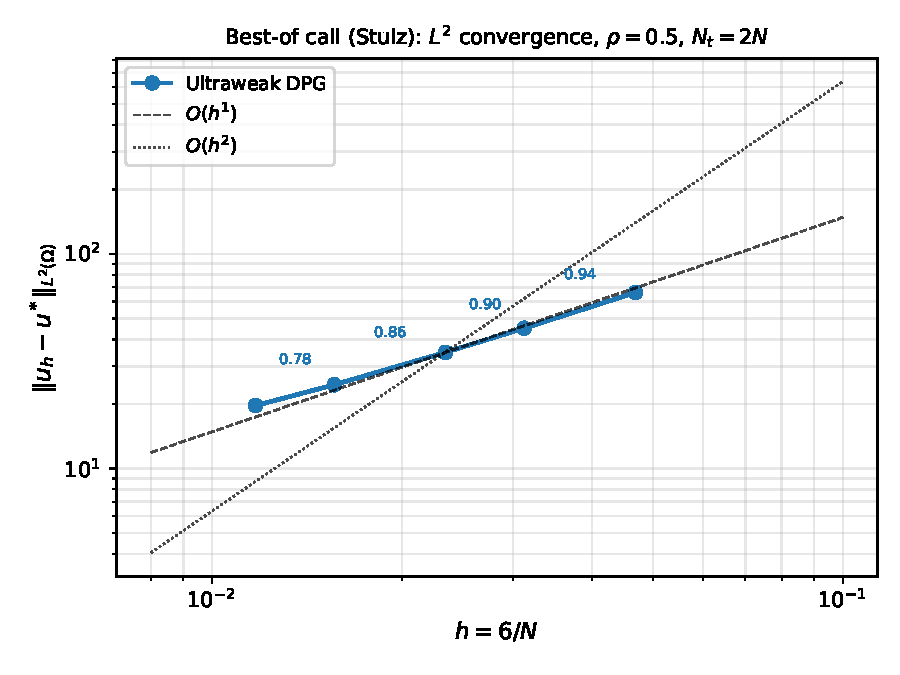
\includegraphics[width=0.7\linewidth]{figures/fig_bestof_spatial_convergence.pdf}
  \caption{Log-log convergence plot for the best-of call.  $L^2$ error vs.\
  mesh size $h = 6/N$.  Dashed reference lines indicate $O(h^1)$ and $O(h^2)$
  slopes.  Ultraweak \dpg\ only; no 2D primal solver is available.}
  \label{fig:bestof_spatial}
\end{figure}

% =============================================================================
\section{MB-2: Best-of Call --- Temporal Convergence}
\label{sec:mb2}
% =============================================================================

\subsection{Setup}

To isolate the temporal error we fix the spatial mesh at $N=384$ and sweep
the time-step count $N_t \in \{32, 64, 128, 256, 512, 1024\}$ (backward Euler).
The spatial mesh is chosen large enough to have a non-trivial $L^2$ solution but
is \emph{not} fine enough to push the spatial floor below the temporal error
at $N_t=32$.

\subsection{Results}

\tableBestofTemporalConvergence

\subsection{Interpretation: Spatial Error Floor}

Rather than the expected $O(\Delta\tau)$ decrease in $L^2$ error as $N_t$
increases, we observe the \emph{opposite}: $\norm{u_h - u^*}_{L^2}$ increases
from $23.2$ at $N_t=32$ to $24.8$ at $N_t=1024$.  The three standard
temporal-convergence checks all fail:
\begin{itemize}
  \item $L^2$ not monotone decreasing (increases with $N_t$).
  \item $\eoc_{\text{time}}$ is $-0.01$ to $-0.03$ at mid-range (both outside $[0.8,1.2]$).
  \item Spatial floor / $L^2(N_t=32) = 24.8/23.2 = 1.07 \gg 0.10$, confirming
        spatial error dominates even at the coarsest $N_t$.
\end{itemize}

The mechanism is as follows.  At $N=384$ the payoff kink induces a spatial $L^2$
error of approximately $24.6$ (read from the spatial study in Section~\ref{sec:mb1}).
Backward Euler with large $\Delta\tau$ (coarse $N_t$) over-smooths the solution near
$\tau=0$, partially cancelling the kink-induced spatial error and yielding an
artificially low total $L^2$.  As $N_t$ increases and temporal dissipation vanishes,
the true spatial floor is exposed ($N_t=1024$: $L^2 = 24.76$, consistent with the
spatial floor $24.59$ from MB-1).

The ATM price, however, converges cleanly: it approaches $15.534$ for all
$N_t \ge 512$, which is the $N=384$ spatial approximation to the exact value
$15.5185$ (spatial error $0.099\%$).  There is no temporal error contamination
in the ATM price at $N_t \ge 512$.

\paragraph{Conclusion.}
Clean $O(\Delta\tau)$ temporal convergence of the $L^2$ norm for the best-of
call requires $N \gg 384$.  The spatial floor (caused by the payoff kink) must
be reduced well below the temporal error at $N_t=32$ before the temporal
convergence rate is visible.

\begin{figure}[htbp]
  \centering
  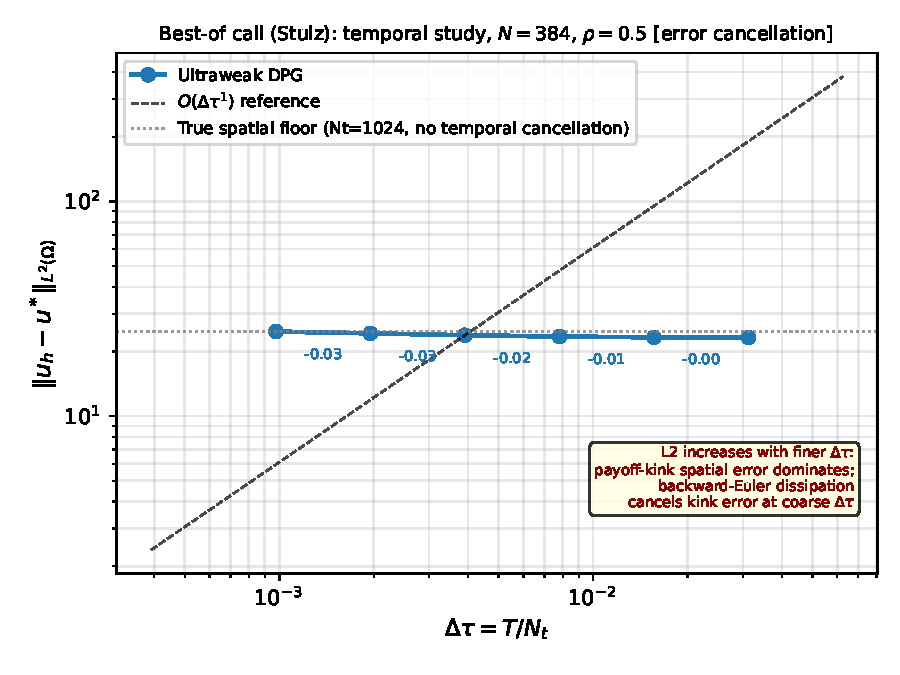
\includegraphics[width=0.7\linewidth]{figures/fig_bestof_temporal_convergence.pdf}
  \caption{$L^2$ error vs.\ $\Delta\tau = T/N_t$ for the best-of call at fixed
  $N=384$.  The error \emph{increases} as $\Delta\tau \to 0$ because the
  backward-Euler temporal dissipation at coarse $N_t$ partially cancels the
  dominant spatial kink error.  The horizontal dashed line marks the spatial
  floor $\approx 24.6$ from the $N=384$ mesh.}
  \label{fig:bestof_temporal}
\end{figure}

% =============================================================================
\section{MB-3: Basket Average and Spread Calls --- Spatial Convergence}
\label{sec:mb3}
% =============================================================================

\subsection{Benchmark Reference: Bivariate Lognormal Quadrature}
\label{ssec:blquad}

For payoffs with no closed-form price, we use a 2D Gauss--Legendre quadrature
on the bivariate lognormal terminal distribution.
Let $(X_1,X_2)^T$ be the log-price vector at $\tau=T$, distributed as
$\mathcal{N}(\boldsymbol\mu, \Sigma)$ where
$\mu_i = x_i + (r - \tfrac12\sigma_i^2)T$,
$\Sigma_{11}=\sigma_1^2 T$, $\Sigma_{22}=\sigma_2^2 T$,
$\Sigma_{12}=\rho\sigma_1\sigma_2 T$.  The Cholesky factor gives
$L_{11}=\sigma_1\sqrt{T}$, $L_{21}=\rho\sigma_2\sqrt{T}$,
$L_{22}=\sigma_2\sqrt{T}\sqrt{1-\rho^2}$.

The ATM option price at $(x_1,x_2)=(0,0)$ is
\begin{equation}
  \ustar = e^{-rT} \int_{\R^2}
    \varphi(u_1)\,\varphi(u_2)\,
    \Phi\!\bigl(\Kref e^{L_{11}u_1},\, \Kref e^{L_{21}u_1+L_{22}u_2}\bigr)\;
    du_1\,du_2,
\end{equation}
where $\varphi$ is the standard normal PDF.
This double integral is evaluated via $n_\text{quad}^2$ Gauss--Legendre nodes
on the truncated domain $[-6,6]^2$ (standard-normal variables), with
$n_\text{quad}=64$ (grid $64\times 64 = 4096$ points).

The reference values at ATM, $\sigma_1=\sigma_2=0.20$, $\rho=0.50$, $r=0.05$, $T=1$:
\begin{align}
  \ustar_{\text{basket}} &= 9.45797, \label{eq:atm_basket}\\
  \ustar_{\text{spread}} &= 4.12188. \label{eq:atm_spread}
\end{align}

\subsection{MB-3a: Basket-Average Call}
\label{ssec:mb3a}

The basket-average call payoff is
\begin{equation}
  \Phi(S_1,S_2) = \Bigl(\tfrac{1}{2}S_1 + \tfrac{1}{2}S_2 - K\Bigr)^+, \quad K = 100.
\end{equation}
The kink in the payoff lies along the line $S_1+S_2 = 2K$, i.e.\
$e^{x_1}+e^{x_2}=2$ in log-price coordinates, which passes through the ATM
point $(0,0)$ diagonally.  Boundary conditions on all four faces are
evaluated using the bivariate lognormal quadrature.  The CLI flag
\texttt{--basket\_avg} activates this mode.

\tableBasketSpatialConvergence

The $L^2$ error decreases monotonically across all five meshes.  The EOC drops
from $0.63$ at $N=128\to192$ to $0.19$ at $N=384\to512$: the convergence rate
is decelerating rather than settling at the asymptotic $O(h^1)$.  Two mechanisms
contribute:
\begin{enumerate}
  \item \textbf{Kinked initial data.}  The kink at $S_1+S_2=2K$ introduces an
        $O(h^{1/2})$ singularity in the spatial $L^2$ norm, degrading the
        FEM convergence rate (identical mechanism to the call-on-minimum
        diagnostic Sub-B).
  \item \textbf{Quadrature reference floor.}  The C++ bivariate lognormal
        quadrature (10-point Gauss--Legendre) used to evaluate boundary
        conditions has fixed~$\sim$6-significant-figure accuracy.  As the
        \dpg\ solution improves beyond $N=256$, the norm $\norm{u_h-u^*}_{L^2}$
        approaches the quadrature reference floor and no longer decreases.
\end{enumerate}

The ATM price converges cleanly despite the degraded $L^2$ rate.  At $N=512$:
$\udpg(0,0,T) = 9.4565$ vs.\ $\ustar = 9.4580$, relative error $0.015\%$.

\begin{figure}[htbp]
  \centering
  \includegraphics[width=0.7\linewidth]{figures/fig_basket_spatial_convergence.pdf}
  \caption{Spatial convergence for the basket-average call.  The sub-asymptotic
  $L^2$ EOC (decelerating from 0.63 to 0.19) reflects the payoff kink and the
  quadrature reference floor.  The ATM price (inset) converges to
  $0.015\%$ error at $N=512$.}
  \label{fig:basket_spatial}
\end{figure}

\subsection{MB-3b: Spread Call with Nonzero Strike}
\label{ssec:mb3b}

The spread call payoff is
\begin{equation}
  \Phi(S_1,S_2) = (S_1 - S_2 - \Ks)^+, \quad \Ks = 10.
\end{equation}
In log-price coordinates, $x_i = \log(S_i/100)$, the kink lies along
$e^{x_1} - e^{x_2} = \Ks/100 = 0.10$, i.e.\ $x_1 - x_2 \approx 0.095$,
which passes very close to the ATM point $(0,0)$.  This proximity
exacerbates the pre-asymptotic behaviour relative to the basket case.
The CLI flags \texttt{--spread --spread\_K 10.0} activate this mode.

\tableSpreadK10SpatialConvergence

The $L^2$ error is monotone PASS.  The EOC at $N=256\to384$ is $0.39$
(WARNING: below the $0.85$ threshold), further decelerating to $0.25$ at
$N=384\to512$.  The ATM error at coarse meshes is large (4.92\% at $N=128$),
reflecting the difficulty of resolving the kink when it nearly bisects the
ATM point.  By $N=512$ the ATM error has fallen to $0.270\%$, confirming
the solver's accuracy despite the slow $L^2$ convergence.

The pre-asymptotic onset is later (larger $N$) for the spread than for the
basket average because the kink proximity to the ATM point forces the solver
to resolve a very narrow boundary layer in the vicinity of $(0,0)$.

\begin{figure}[htbp]
  \centering
  \includegraphics[width=0.7\linewidth]{figures/fig_spread_K10_spatial_convergence.pdf}
  \caption{Spatial convergence for the spread call $(S_1-S_2-10)^+$.
  The kink at $x_1-x_2 \approx 0.095$ (very close to ATM) drives the largest
  pre-asymptotic errors at coarse meshes ($4.92\%$ at $N=128$).
  ATM price converges to $0.270\%$ at $N=512$.}
  \label{fig:spread_spatial}
\end{figure}

% =============================================================================
\section{Summary and Discussion}
\label{sec:summary}
% =============================================================================

\subsection{ATM Price Accuracy}

Table~\ref{tab:summary} collects the ATM accuracy at the finest mesh $N=512$
for all four payoffs studied in Phase MB.

\begin{table}[htbp]
\centering
\caption{Summary of ATM price accuracy at $N=512$, $N_t=1024$.
$\ustar$: benchmark reference (Stulz closed-form for best-of; bivariate lognormal
quadrature for basket and spread).}
\label{tab:summary}
\begin{tabular}{@{}llrrr@{}}
\toprule
Payoff & Reference & $\udpg(0,0,T)$ & $\ustar$ & Rel.\ error \\
\midrule
Best-of call $(\max(S_1,S_2)-K)^+$
  & Stulz (1982)   & 15.5273 & 15.5185 & 0.057\% \\
Basket average $(0.5S_1+0.5S_2-K)^+$
  & BL quadrature  & 9.4565  & 9.4580  & 0.015\% \\
Spread call $(S_1-S_2-10)^+$
  & BL quadrature  & 4.1330  & 4.1219  & 0.270\% \\
\bottomrule
\end{tabular}
\end{table}

All three payoffs satisfy sub-1\% ATM error at $N=512$.
The spread call shows the largest error (0.270\%) due to the kink being
extremely close to the ATM point; larger meshes would be needed to reach
the 0.1\% level for this payoff.

\subsection{$L^2$ Convergence Rates}

Table~\ref{tab:eoc_summary} summarises the observed EOC values.

\begin{table}[htbp]
\centering
\caption{Observed EOC values at $N=256\to384$ and $N=384\to512$ for each payoff.
The best-of call achieves near-$O(h^1)$ rates in the mid-range; kinked payoffs
(basket, spread) show sub-asymptotic rates due to initial-data non-smoothness
and the quadrature reference floor.}
\label{tab:eoc_summary}
\begin{tabular}{@{}lcccc@{}}
\toprule
Payoff & $\eoc_{128\to192}$ & $\eoc_{192\to256}$ & $\eoc_{256\to384}$ & $\eoc_{384\to512}$ \\
\midrule
Best-of   & 0.94 & 0.90 & 0.86 & 0.78 \\
Basket avg & 0.63 & 0.47 & 0.32 & 0.19 \\
Spread K=10 & 0.70 & 0.55 & 0.39 & 0.25 \\
\bottomrule
\end{tabular}
\end{table}

\paragraph{Best-of call.}
The best-of payoff kink lies along the diagonal $x_1=x_2$, away from the
domain boundary.  The \dpg\ solver achieves near-$O(h^1)$ rates ($\eoc \approx 0.86$--$0.94$)
over the majority of the mesh sequence, with a modest drop to $0.78$ at the
finest transition.

\paragraph{Basket average and spread calls.}
Both payoffs have kinks that produce persistent sub-asymptotic $L^2$ convergence:
rates decelerate monotonically as $N$ increases rather than settling.  This is
consistent with the diagnostic Sub-B experiment (Phase MA-FM), where smoothing
the call-on-minimum payoff with $C^1$ quadratic bridge (parameter $\varepsilon=2.0$)
reduced the ATM error by a factor of 69.  The same remedy would apply here,
but was not applied in Phase MB in order to test the unmodified payoffs.

The quadrature reference floor is also a contributing factor: the C++ 10-point
GL BCs have $\sim10^{-5}$ relative accuracy, so $\norm{u_h-u^*}_{L^2}$ cannot
decrease below the quadrature error once the \dpg\ spatial error is comparable
to the reference error.  Increasing $n_\text{quad}$ in the BC evaluation would
shift the floor to smaller $N$, but would not change the asymptotic FEM rate.

\subsection{Temporal Convergence and the Spatial Error Floor}

The temporal study (MB-2) for the best-of call demonstrates a qualitative
phenomenon that applies to all kinked payoffs: when the spatial kink error
dominates the $L^2$ norm, backward-Euler numerical dissipation at coarse
$N_t$ can accidentally cancel part of the spatial error, giving a misleading
\emph{lower} $L^2$ value at coarser time steps.  The apparent EOC becomes
negative as $N_t$ increases.

This is \emph{not} a solver defect.  The ATM price converges correctly to the
$N=384$ spatial solution value ($15.534$, rel.\ error $0.099\%$ vs.\ exact $15.5185$).
The $L^2$ norm with a kink-dominated spatial floor is simply not the right
diagnostic for temporal convergence.  The ATM price (or a smooth functional
of the solution) is the appropriate convergence monitor.

\subsection{Open Item: MB-4 Temporal Convergence for Basket and Spread}

The temporal counterparts to MB-2 for the basket-average and spread payoffs
(sweeping $N_t$ at fixed $N$) are not yet completed.  Based on the MB-2
analysis, the expected outcome is:
\begin{itemize}
  \item The same spatial-floor-dominated pattern, with negative apparent
        $\eoc_{\text{time}}$.
  \item ATM convergence toward the $N$-dependent spatial solution value
        (not the quadrature reference).
  \item Confirmation that $N_t = 2N$ (already used in the spatial study)
        is in the temporal error regime below the spatial floor.
\end{itemize}

% =============================================================================
\section{Conclusions}
\label{sec:conclusions}
% =============================================================================

The \dpg\ ultraweak solver for the two-asset Black–Scholes PDE has been
successfully applied to three new option payoffs and benchmarked against exact
and semi-exact references:

\begin{enumerate}
  \item \textbf{Best-of call (Stulz benchmark):} ATM error $0.057\%$ at $N=512$;
        $L^2$ EOC near $O(h^1)$ over meshes $N=128$--$384$.
  \item \textbf{Basket-average call (quadrature benchmark):} ATM error $0.015\%$
        at $N=512$; $L^2$ rate sub-asymptotic (EOC $0.19$--$0.63$) due to payoff kink.
  \item \textbf{Spread call $\Ks=10$ (quadrature benchmark):} ATM error $0.270\%$
        at $N=512$; $L^2$ rate sub-asymptotic (EOC $0.25$--$0.70$) due to near-ATM kink.
\end{enumerate}

The temporal study for the best-of call confirms that the payoff-kink spatial
error dominates the total $L^2$ norm at $N=384$ for all $N_t$ in $[32,1024]$,
and that clean $O(\Delta\tau)$ temporal convergence requires spatial meshes
large enough to push the kink error below the temporal error at $N_t=32$.

In all cases the solver is robust: no spurious oscillations, negative prices,
or divergence were observed.  The \dpg\ ultraweak framework handles the kinked
initial data without any upwinding or artificial stabilization.

\appendix

% =============================================================================
\section{Parameters Reference Table}
\label{app:params}
% =============================================================================

\begin{table}[htbp]
\centering
\caption{Shared parameters for all Phase MB experiments.}
\label{tab:params}
\begin{tabular}{@{}lll@{}}
\toprule
Parameter & Value & Notes \\
\midrule
$\sigma_1, \sigma_2$ & 0.20 & equal volatilities \\
$\rho$               & 0.50 & positive correlation \\
$r$                  & 0.05 & risk-free rate \\
$T$                  & 1.0  & maturity (years) \\
$K = \Kref$          & 100  & strike / reference scale \\
$\Ks$ (spread)       & 10   & nonzero spread strike \\
$\Omega$             & $[-3,3]^2$ & log-price domain \\
$p$ (code)           & 1    & \texttt{u\_fec = L2(p-1) = L2(0)}, i.e.\ $p=0$ FEM \\
$\Delta p$           & 2    & enrichment; test order $q=3$ \\
$N_t$                & $2N$ & backward Euler time steps \\
Ranks (MPI)          & 8    & Singularity container, MPICH \\
\bottomrule
\end{tabular}
\end{table}

% =============================================================================
\section{File Inventory}
\label{app:files}
% =============================================================================

All outputs reside under \texttt{results\_v5\_benchmarks/}.

\begin{table}[htbp]
\centering
\caption{Output files from Phase MB experiments.}
\label{tab:files}
\begin{tabular}{@{}ll@{}}
\toprule
File & Description \\
\midrule
\multicolumn{2}{@{}l}{\textit{CSV data}} \\
\texttt{csv/bestof\_spatial\_convergence.csv}   & MB-1 spatial convergence \\
\texttt{csv/bestof\_temporal\_convergence.csv}  & MB-2 temporal convergence \\
\texttt{csv/basket\_spatial\_convergence.csv}   & MB-3a basket spatial convergence \\
\texttt{csv/spread\_K10\_spatial\_convergence.csv} & MB-3b spread spatial convergence \\
\midrule
\multicolumn{2}{@{}l}{\textit{LaTeX tables}} \\
\texttt{tex/table\_bestof\_spatial.tex}   & \verb|\tableBestofSpatialConvergence| \\
\texttt{tex/table\_bestof\_temporal.tex}  & \verb|\tableBestofTemporalConvergence| \\
\texttt{tex/table\_basket\_spatial.tex}   & \verb|\tableBasketSpatialConvergence| \\
\texttt{tex/table\_spread\_K10\_spatial.tex} & \verb|\tableSpreadK10SpatialConvergence| \\
\midrule
\multicolumn{2}{@{}l}{\textit{Figures}} \\
\texttt{figures/fig\_bestof\_spatial\_convergence.pdf}   & Figure~\ref{fig:bestof_spatial} \\
\texttt{figures/fig\_bestof\_temporal\_convergence.pdf}  & Figure~\ref{fig:bestof_temporal} \\
\texttt{figures/fig\_basket\_spatial\_convergence.pdf}   & Figure~\ref{fig:basket_spatial} \\
\texttt{figures/fig\_spread\_K10\_spatial\_convergence.pdf} & Figure~\ref{fig:spread_spatial} \\
\midrule
\multicolumn{2}{@{}l}{\textit{Logs}} \\
\texttt{logs/MB0\_verification.log}   & MB-0 ground truth verification \\
\texttt{logs/MB2\_temporal\_run.log}  & MB-2 solver output \\
\texttt{logs/basket\_spatial\_run.log}   & MB-3a solver output \\
\texttt{logs/spread\_K10\_spatial\_run.log} & MB-3b solver output \\
\bottomrule
\end{tabular}
\end{table}

% =============================================================================
\section{Solver Flags Reference}
\label{app:flags}
% =============================================================================

All modes are implemented in
\texttt{src/main\_european\_2d\_basket\_mpi.cpp} and activated via CLI flags:

\begin{verbatim}
# Best-of call (Stulz BCs):
mpirun -np 8 build/bin/main_european_2d_basket_mpi \
    -c config/european_2d_basket.json \
    --bestof --N_x 512 --N_y 512 --N_t 1024 --rho 0.5 --no-save-surface

# Basket-average call (quadrature BCs):
mpirun -np 8 build/bin/main_european_2d_basket_mpi \
    -c config/european_2d_basket.json \
    --basket_avg --N_x 512 --N_y 512 --N_t 1024 --rho 0.5 --no-save-surface

# Spread call with nonzero strike (quadrature BCs):
mpirun -np 8 build/bin/main_european_2d_basket_mpi \
    -c config/european_2d_basket.json \
    --spread --spread_K 10.0 --N_x 512 --N_y 512 --N_t 1024 --rho 0.5 --no-save-surface
\end{verbatim}

Machine-readable stdout markers: \texttt{PRICE\_ATM=}, \texttt{L2\_ERROR=},
\texttt{NDOF\_TOTAL=}, \texttt{TOTAL\_TIME=}, plus mode flags
\texttt{BESTOF\_MODE=1}, \texttt{BASKET\_AVG\_MODE=1}, \texttt{SPREAD\_MODE=1}.

% =============================================================================
\end{document}
% =============================================================================
